\begin{figure}[H]
\centering
\begin{minipage}[t]{58mm}
\vspace{0pt}
\centering
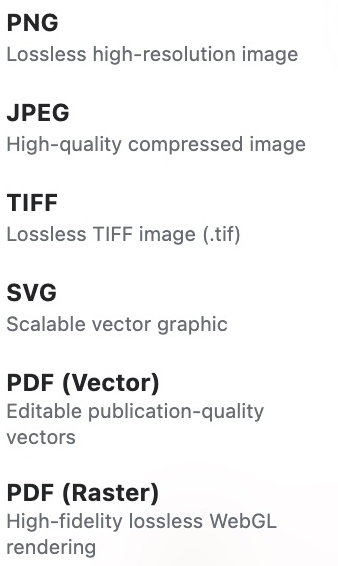
\includegraphics[width=52mm]{publication-assets/crop-496bc1fbfb3e99bfc4e7.png}
\end{minipage}\hspace{4mm}%
\begin{minipage}[t]{58mm}
\vspace{0pt}
{\centering
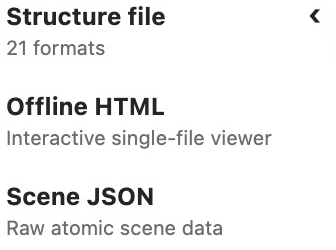
\includegraphics[width=51mm]{publication-assets/crop-68b4df9ea7d48ce9da1e.png}\par}
\par\vspace{3mm}
\raggedright\fontsize{9}{13}\selectfont
\ui{Structure file} saves the model information supported by the selected format.

\smallskip
\ui{Offline HTML} provides an interactive view in a local browser.

\smallskip
\ui{Scene JSON} records the atomic scene and is distinct from structure JSON.
\end{minipage}
\caption{The atomic viewer's export menus. \ui{Export image} on the left offers six image formats. \ui{Export file} on the right provides structure files, an offline page, and scene JSON.}
\label{fig:atomic-export-menus}
\end{figure}
